% British English Proficiency Programme — Vowels chapter
% Compile standalone with: pdflatex british_english_vowels_chapter.tex (twice)
% For master book: define \VowelsStandalonefalse before \input{...}.
% \ifdefined\VowelsStandalonefalse\else
% \documentclass[11pt,a4paper,oneside]{book}
% \usepackage{fontspec}
% \setmainfont{DejaVu Serif}
% \setmonofont{DejaVu Sans Mono}
% \usepackage[british]{babel}

% \usepackage{geometry}
% \geometry{margin=27mm}
% \usepackage{longtable,booktabs,array,tabularx,multicol,enumitem}
% \usepackage{xcolor,graphicx,hyperref,fancyhdr,tcolorbox}
% \tcbuselibrary{breakable,skins}
% \hypersetup{colorlinks=true,linkcolor=blue!45!black,urlcolor=blue!50!black}
% \newcommand{\ipa}[1]{{\fontspec{DejaVu Sans}/#1/}}
% \newcommand{\res}[3]{\begin{tcolorbox}[breakable,colback=gray!5,colframe=gray!55,title={Resource placeholder: #1}]\textbf{Deliverable:} #2\par\textbf{Specification:} #3\end{tcolorbox}}
% \newcommand{\task}[2]{\begin{tcolorbox}[breakable,colback=blue!2,colframe=blue!45!black,title={Practice: #1}]#2\end{tcolorbox}}
% \newcommand{\checkline}{\par\noindent\rule{\linewidth}{0.35pt}\par}
% \setcounter{tocdepth}{2}
% \begin{document}
% \frontmatter
% \title{British English Vowels\\\large A Comprehensive Pronunciation and Listening Laboratory}
% \author{British English Proficiency Programme}
% \date{Curriculum edition 1.0}
% \maketitle
% \tableofcontents
% \mainmatter
% \fi
\chapter{British English Vowels: Perception, Articulation and Fluent Speech}
\label{chap:british-vowels}

\begin{figure}[t]
    \centering
    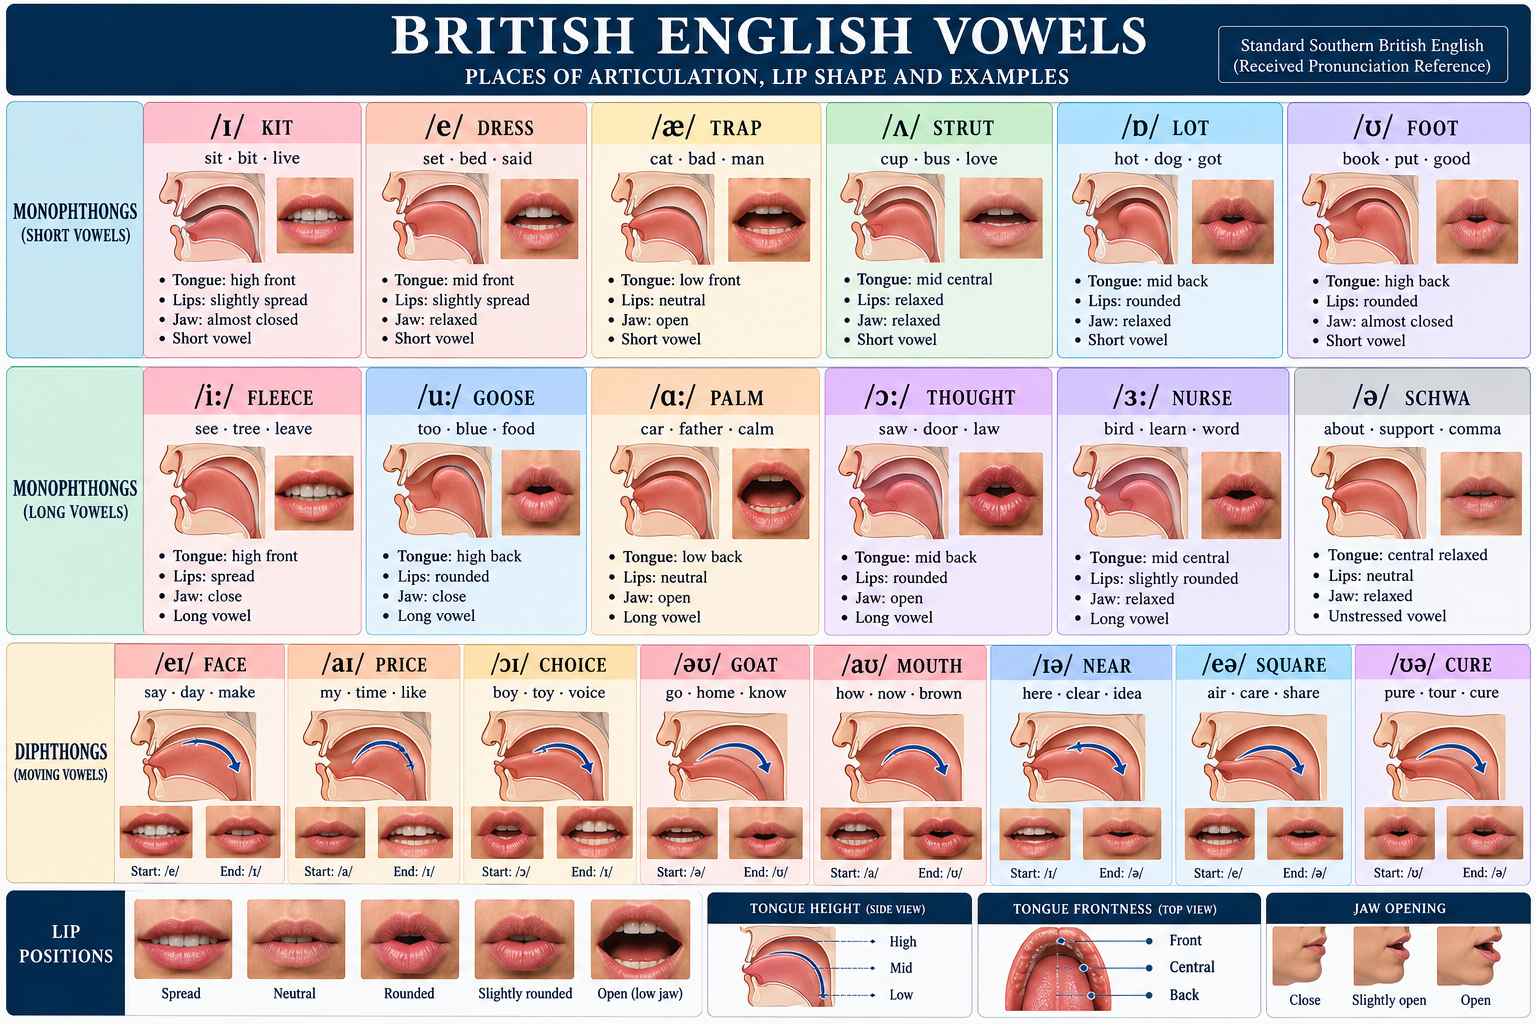
\includegraphics[width=1\linewidth]{images/all-in-one-british-vowels.png}
    \caption{British English vowels postures of the vocal organs}
    \label{fig:british-english-vowels}
\end{figure}

\noindent\textbf{Target accent:} contemporary Standard Southern British English (SSBE), with traditional Received Pronunciation (RP) comparisons.\par
\noindent\textbf{Suggested duration:} 6--8 weeks within a two-hour daily training programme. This is a planning estimate, not a guaranteed proficiency timeline.\par
\noindent\textbf{Prerequisites:} basic understanding of syllables and familiarity with dictionary entries.\par
\section{Learning outcomes}
By the end of this chapter, the learner should be able to (i) recognise the major SSBE vowel categories in isolated and connected speech; (ii) describe and reproduce their articulatory targets; (iii) distinguish important minimal pairs; (iv) recognise weak forms and schwa; (v) interpret broad IPA transcription; and (vi) monitor vowel accuracy during academic and professional communication.
\section{How to use this chapter}
Each vowel laboratory follows the sequence \emph{listen, discriminate, position, produce, contrast, read, record, review}. Do not increase speaking speed until the contrast is reliably audible and producible. Audio prompts are marked as resources and must be recorded or sourced before listening-only tests are administered.
\res{AUD-000}{Master accent reference recording}{One adult SSBE speaker and a second comparison speaker; isolated vowels, lexical-set keywords, slow and natural-speed phrases; lossless WAV and accessible MP3.}
\section{Diagnostic baseline}
Record a 60-second introduction, read the passage below, and pronounce the word pairs \emph{sheep--ship, bed--bad, cut--cart, full--fool, cot--caught, late--light}. Save both unedited audio and a brief self-assessment. The recording is a baseline rather than a pass/fail test.
\task{Baseline reading}{``This week I need to explain the results of our latest experiment. We checked the data, compared the figures and discussed which changes would improve the system. I would like to present a clear summary at the next meeting.'' Record once at normal speed, then annotate the vowels you find difficult.}
\res{REC-001}{Baseline recording form}{Date, microphone conditions, reading time, confidence, target words, observed problems, and link to audio file.}
\section{The physiology of vowels}
Vowels are typically voiced speech sounds produced without a complete closure or a turbulent constriction in the vocal tract. Vowel quality depends strongly on tongue position, lip posture, jaw opening and the resulting vocal-tract resonances. The traditional vowel quadrilateral is an articulatory map, not a literal photograph of the tongue.
\subsection{Height, backness and lip rounding}
\emph{Height} describes the vertical position of the tongue body; \emph{backness} describes its front-to-back position. Rounded lips can lengthen the effective vocal tract and change resonance. Jaw movement and tongue movement are related but not identical.
\res{FIG-001}{Sagittal vocal-tract anatomy}{Label lips, jaw, tongue tip, blade, body and root, hard palate, soft palate, pharynx, and larynx; vector PDF preferred.}
\res{FIG-002}{IPA vowel quadrilateral}{High/mid/low and front/central/back axes, with schematic SSBE vowel locations; include note about speaker variation.}
\res{FIG-003}{Lip and jaw posture plate}{Photographic or schematic front views for spread, neutral, rounded and open positions; matched scale and neutral lighting.}
\subsection{Length, stress and context}
The colon-like length mark \texttt{ː} distinguishes conventional broad transcriptions such as \ipa{iː} from \ipa{ɪ}. Actual duration also varies with stress, speech rate and following consonants. In particular, a vowel is commonly shorter before a fortis consonant than before a lenis consonant: compare \emph{seat} and \emph{seed}. Never rely on duration alone to identify an English vowel.
\res{FIG-004}{Pre-fortis clipping timeline}{Compare the same vowel in seat/seed and beat/bead, with measured examples and speaker metadata; do not fabricate durations.}
\subsection{A note on notation and accent variation}
Broad transcriptions are pedagogical approximations. Modern SSBE may use a fronter GOOSE vowel, variable GOAT onsets, and monophthongal pronunciations in words historically transcribed with centring diphthongs. The traditional RP CURE category \ipa{ʊə} is often merged with THOUGHT \ipa{ɔː} in common words such as \emph{sure}; NEAR and SQUARE may also vary. Learn the reference model, then recognise variants without treating every difference as an error.
\section{The vowel inventory}
\begin{longtable}{lll p{0.38\linewidth}}
\toprule Class & Lexical set & Broad IPA & Keyword and note\\\midrule\endhead
Short & KIT & \ipa{ɪ} & kit\\
Short & DRESS & \ipa{e} & dress\\
Short & TRAP & \ipa{æ} & trap\\
Short & STRUT & \ipa{ʌ} & strut\\
Short & LOT & \ipa{ɒ} & lot\\
Short & FOOT & \ipa{ʊ} & foot\\
Long & FLEECE & \ipa{iː} & fleece\\
Long & GOOSE & \ipa{uː} & goose\\
Long & PALM & \ipa{ɑː} & palm\\
Long & THOUGHT & \ipa{ɔː} & thought\\
Long & NURSE & \ipa{ɜː} & nurse\\
Weak & commA & \ipa{ə} & about, comma (unstressed)\\
Diphthong & FACE & \ipa{eɪ} & face\\
Diphthong & PRICE & \ipa{aɪ} & price\\
Diphthong & CHOICE & \ipa{ɔɪ} & choice\\
Diphthong & GOAT & \ipa{əʊ} & goat (traditional broad SSBE)\\
Diphthong & MOUTH & \ipa{aʊ} & mouth\\
Variable centring & NEAR & \ipa{ɪə} & near; modern variants exist\\
Variable centring & SQUARE & \ipa{eə} & square; modern variants exist\\
Variable centring & CURE & \ipa{ʊə} & cure; limited and variable in modern SSBE\\
\bottomrule
\end{longtable}
\res{FIG-005}{Master vowel chart poster}{All lexical sets, IPA, example words, colour-coded categories, and centring-diphthong variation warning; A3 printable PDF and SVG.}

\section{Preparatory articulation gym}

\begin{enumerate}[label=\arabic*.]
\item \textbf{Jaw release (60 s):} alternate relaxed closed-mouth posture and comfortable opening without forcing the joint.
\item \textbf{Lip alternation (60 s):} move gently between spread, neutral and rounded lips without voicing.
\item \textbf{Tongue awareness (90 s):} alternate a high-front and a high-back tongue-body position; avoid pressing against the palate.
\item \textbf{Sustained voicing (60 s):} sustain a comfortable vowel for several seconds, keeping the pitch and loudness stable.
\item \textbf{Vowel-space ladder (3 min):} repeat \ipa{iː}--\ipa{ɪ}--\ipa{e}--\ipa{æ}--\ipa{ɑː}, slowly and without inserting consonants.
\item \textbf{Rounding ladder (3 min):} contrast \ipa{uː}, \ipa{ʊ}, \ipa{ɔː}, \ipa{ɒ}; use a mirror to notice the lips.
\item \textbf{Silent-to-voiced transfer (2 min):} form the target mouth shape silently, then voice it without shifting position.
\end{enumerate}

Stop any movement that causes pain or strain; exaggerated articulation is a temporary training aid, not a speaking goal.
\res{VID-001}{Articulatory warm-up demonstration}{Close-up front and side videos with slow motion, subtitles and accessible verbal instructions.}
\task{Preparation checklist}{Mark each as comfortable / uncertain / difficult: lip rounding, jaw opening, high-front tongue, back-vowel posture, steady voicing, and silent-to-voiced transfer. Repeat uncertain movements before the next laboratory.}

\section{KIT: \ipa{ɪ}}
\label{sec:vowel-01}

\begin{figure}[H]
    \centering
    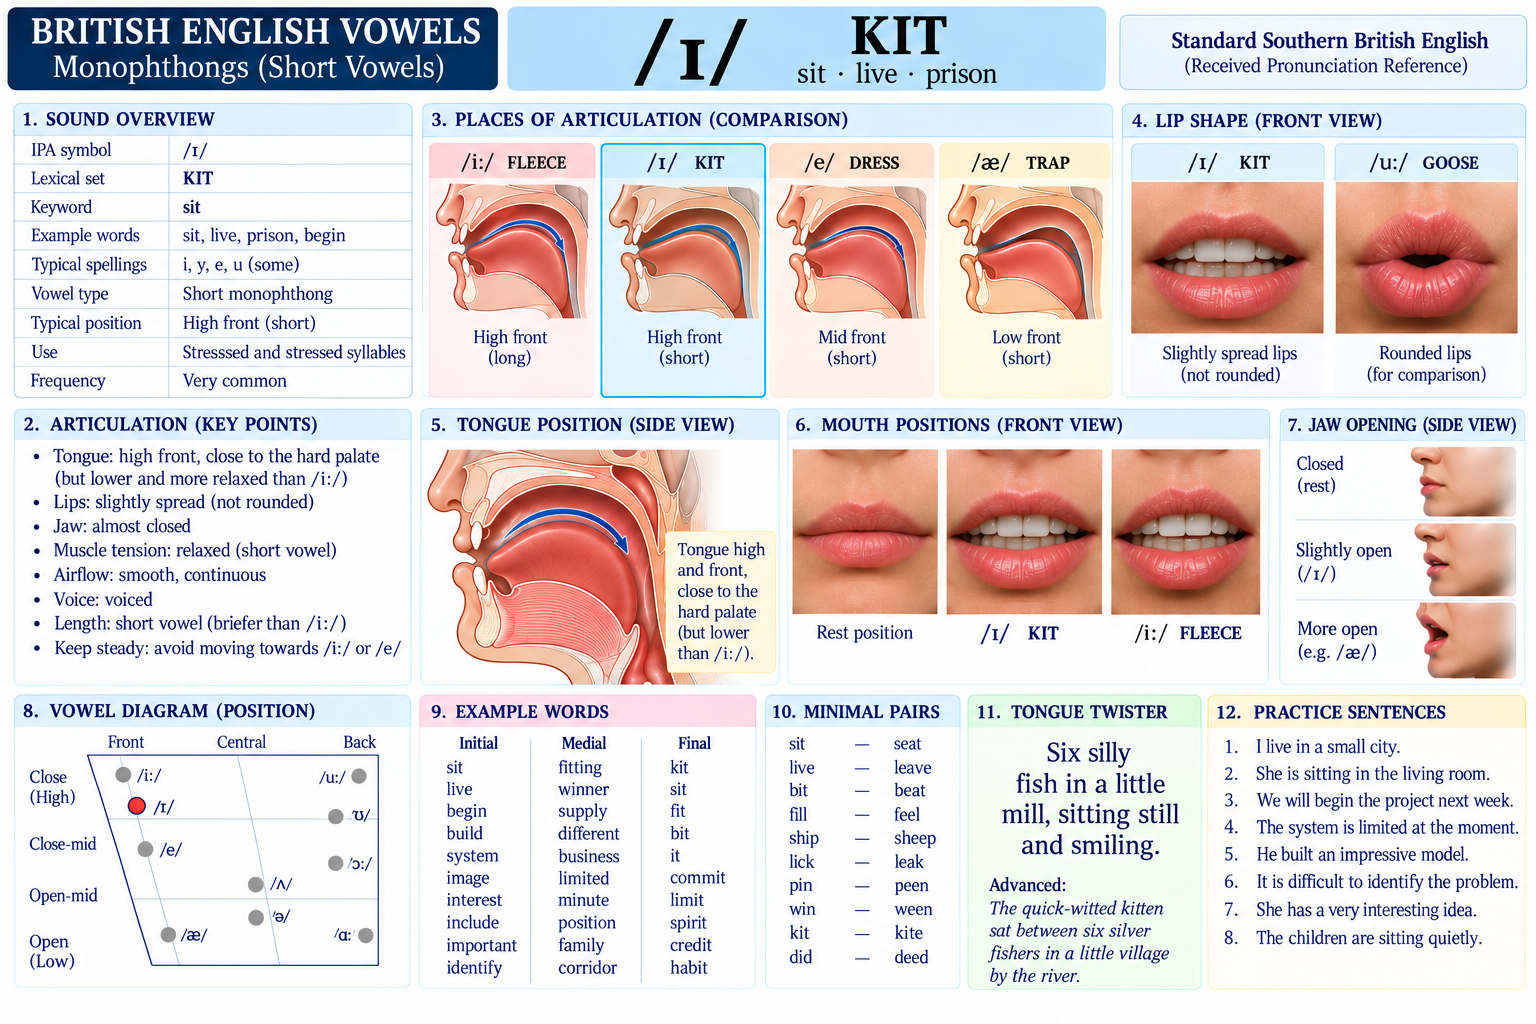
\includegraphics[width=1\linewidth]{images/vowel-ii.png}
    \caption{Enter Caption}
    \label{fig:placeholder}
\end{figure}
\textbf{Lexical anchor:} kit. \textbf{Core examples:} sit, ship, live, rich, fill.\par
\textbf{Articulatory target:} Keep the tongue near-high and front; the vowel is typically more central and lax than FLEECE. Observe tongue-body placement, lip posture and jaw aperture; compare your recording with the reference speaker rather than using spelling as a guide.
\res{FIG-101}{KIT articulation plate}{Front and sagittal views, highlighted tongue target and lips, vowel-map dot, and comparison with nearest category; SVG and PDF.}
\res{AUD-101}{KIT native-speaker model}{Isolated target (three repetitions), each example word (slow/natural), minimal-pair contrasts, phrase, sentence and tongue twister; WAV/MP3, transcript and speaker metadata.}
\subsection{Perception and discrimination}
\task{Hear the difference}{Use the companion audio. For ten randomised trials, identify the target vowel or the contrasting vowel. Write your choice and confidence (1--5). Include at least two repeated items to check consistency. No answer can be scored until the audio stimulus list is supplied.}
\res{LST-101}{KIT discrimination test}{Ten balanced, randomised tokens with answer key, trial order, lexical context and no visible words during listening.}
\subsection{Production ladder}
\begin{enumerate}[label=\arabic*.]
\item Sustain \ipa{ɪ} gently three times; compare with the model.
\item Say each core example in isolation, then embed it in ``I said \emph{[word]} clearly.''
\item Practise the contrasts: sheep--ship; leave--live; feel--fill.
\item Repeat each contrast at slow, conversational and presentation speeds.
\item Record the sentence below and listen for target-vowel consistency.
\end{enumerate}
\textbf{Controlled sentence:} Six little ships slipped into the mist.
\subsection{Tongue-twister laboratory}
Say the controlled sentence three times accurately, then twice at natural speed. Mark any vowel that shifts category. Speed is secondary to intelligibility.
\subsection{Reading and transfer}
\task{Mini-reading and spontaneous transfer}{Read the following original prompt aloud, then speak for 30--45 seconds without a script: ``Explain a recent decision, the evidence behind it, and the next action.'' Insert at least three words from this vowel laboratory. Underline them in your transcript and review their pronunciation.}
\res{TXT-101}{KIT graded reading}{A 100--150-word original passage with 12--20 instances of the target vowel, marked and unmarked versions, vocabulary glosses and comprehension questions.}
\res{REC-101}{KIT recording worksheet}{Word checklist, contrast accuracy, vowel stability, speaking-rate notes, self-correction and tutor feedback.}

\section{DRESS: \ipa{e}}
\label{sec:vowel-02}

\begin{figure}[H]
    \centering
    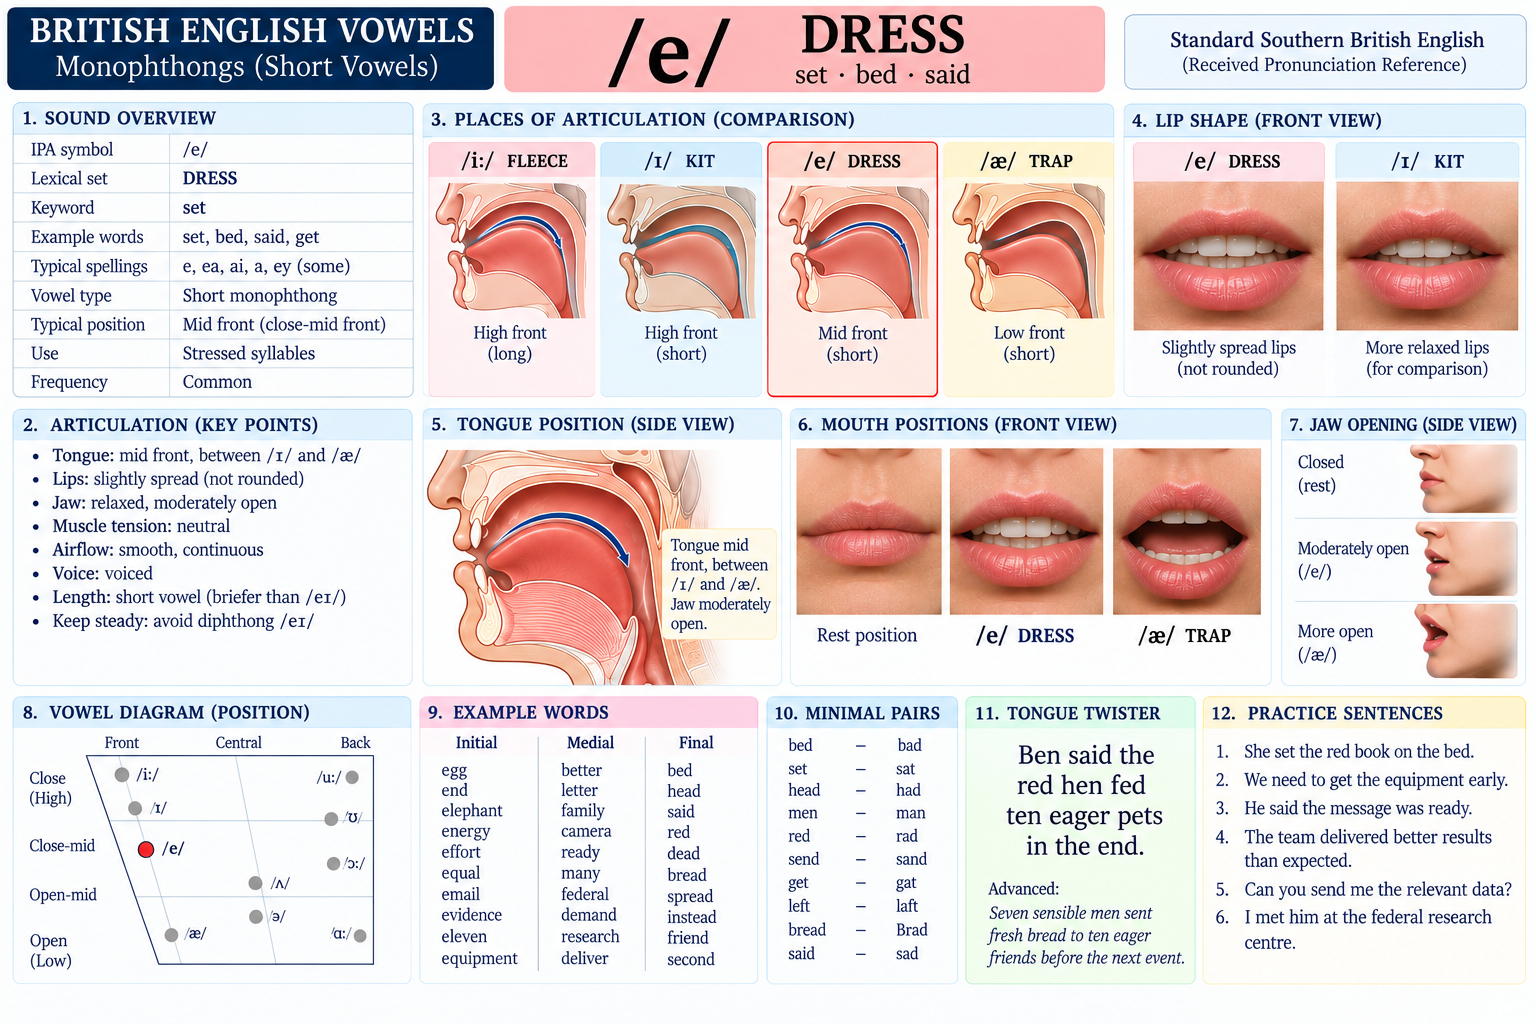
\includegraphics[width=1\linewidth]{images/vowel-e.png}
    \caption{Vowel \ipa{e} construction}
    \label{fig:placeholder}
\end{figure}

\textbf{Lexical anchor:} dress. \textbf{Core examples:} bed, head, said, ten, send.\par
\textbf{Articulatory target:} Use a mid-front tongue position with relatively neutral lips. Observe tongue-body placement, lip posture and jaw aperture; compare your recording with the reference speaker rather than using spelling as a guide.
\res{FIG-102}{DRESS articulation plate}{Front and sagittal views, highlighted tongue target and lips, vowel-map dot, and comparison with nearest category; SVG and PDF.}
\res{AUD-102}{DRESS native-speaker model}{Isolated target (three repetitions), each example word (slow/natural), minimal-pair contrasts, phrase, sentence and tongue twister; WAV/MP3, transcript and speaker metadata.}
\subsection{Perception and discrimination}
\task{Hear the difference}{Use the companion audio. For ten randomised trials, identify the target vowel or the contrasting vowel. Write your choice and confidence (1--5). Include at least two repeated items to check consistency. No answer can be scored until the audio stimulus list is supplied.}
\res{LST-102}{DRESS discrimination test}{Ten balanced, randomised tokens with answer key, trial order, lexical context and no visible words during listening.}
\subsection{Production ladder}
\begin{enumerate}[label=\arabic*.]
\item Sustain \ipa{e} gently three times; compare with the model.
\item Say each core example in isolation, then embed it in ``I said \emph{[word]} clearly.''
\item Practise the contrasts: bed--bad; men--man; pen--pan.
\item Repeat each contrast at slow, conversational and presentation speeds.
\item Record the sentence below and listen for target-vowel consistency.
\end{enumerate}
\textbf{Controlled sentence:} Ten clever friends checked the red pens.
\subsection{Tongue-twister laboratory}
Say the controlled sentence three times accurately, then twice at natural speed. Mark any vowel that shifts category. Speed is secondary to intelligibility.
\subsection{Reading and transfer}
\task{Mini-reading and spontaneous transfer}{Read the following original prompt aloud, then speak for 30--45 seconds without a script: ``Explain a recent decision, the evidence behind it, and the next action.'' Insert at least three words from this vowel laboratory. Underline them in your transcript and review their pronunciation.}
\res{TXT-102}{DRESS graded reading}{A 100--150-word original passage with 12--20 instances of the target vowel, marked and unmarked versions, vocabulary glosses and comprehension questions.}
\res{REC-102}{DRESS recording worksheet}{Word checklist, contrast accuracy, vowel stability, speaking-rate notes, self-correction and tutor feedback.}

\section{TRAP: \ipa{æ}}
\label{sec:vowel-03}

\begin{figure}[H]
    \centering
    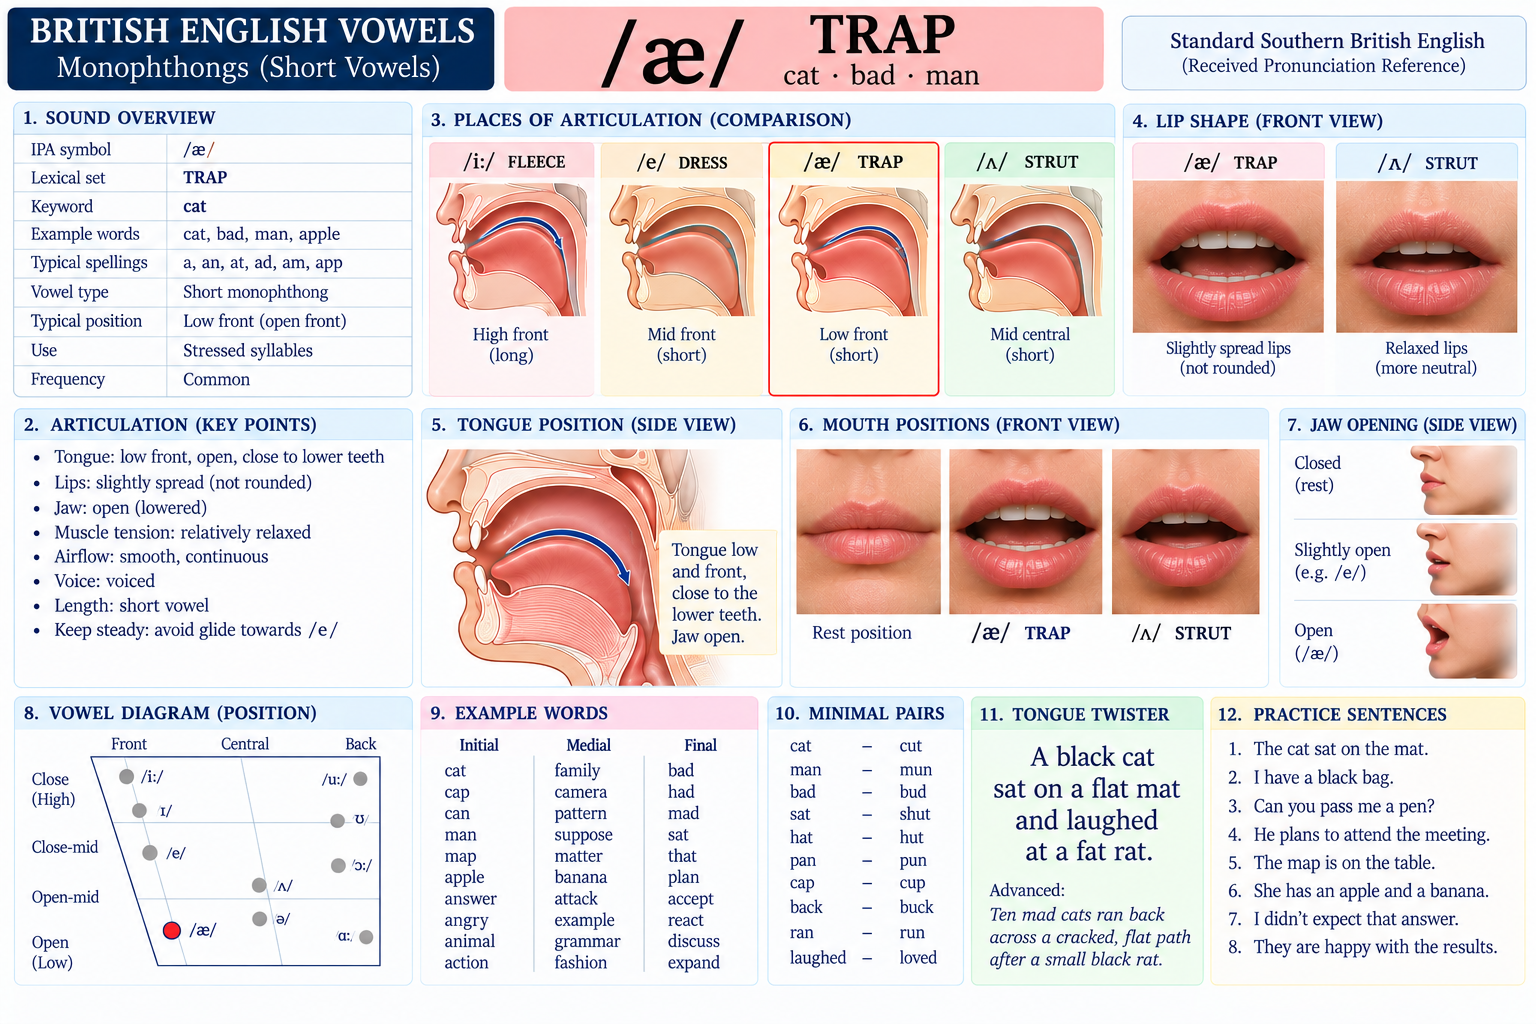
\includegraphics[width=1\linewidth]{images/vowel-ae.png}
    \caption{Vowel \ipa{æ} construction}
    \label{fig:placeholder}
\end{figure}

\textbf{Lexical anchor:} trap. \textbf{Core examples:} cat, bad, map, plan, match.\par
\textbf{Articulatory target:} Lower the front tongue and open the jaw comfortably; avoid replacing it with Spanish /a/. Observe tongue-body placement, lip posture and jaw aperture; compare your recording with the reference speaker rather than using spelling as a guide.
\res{FIG-103}{TRAP articulation plate}{Front and sagittal views, highlighted tongue target and lips, vowel-map dot, and comparison with nearest category; SVG and PDF.}
\res{AUD-103}{TRAP native-speaker model}{Isolated target (three repetitions), each example word (slow/natural), minimal-pair contrasts, phrase, sentence and tongue twister; WAV/MP3, transcript and speaker metadata.}
\subsection{Perception and discrimination}
\task{Hear the difference}{Use the companion audio. For ten randomised trials, identify the target vowel or the contrasting vowel. Write your choice and confidence (1--5). Include at least two repeated items to check consistency. No answer can be scored until the audio stimulus list is supplied.}
\res{LST-103}{TRAP discrimination test}{Ten balanced, randomised tokens with answer key, trial order, lexical context and no visible words during listening.}
\subsection{Production ladder}
\begin{enumerate}[label=\arabic*.]
\item Sustain \ipa{æ} gently three times; compare with the model.
\item Say each core example in isolation, then embed it in ``I said \emph{[word]} clearly.''
\item Practise the contrasts: bad--bed; man--men; hat--hut.
\item Repeat each contrast at slow, conversational and presentation speeds.
\item Record the sentence below and listen for target-vowel consistency.
\end{enumerate}
\textbf{Controlled sentence:} A happy manager mapped the plan.
\subsection{Tongue-twister laboratory}
Say the controlled sentence three times accurately, then twice at natural speed. Mark any vowel that shifts category. Speed is secondary to intelligibility.
\subsection{Reading and transfer}
\task{Mini-reading and spontaneous transfer}{Read the following original prompt aloud, then speak for 30--45 seconds without a script: ``Explain a recent decision, the evidence behind it, and the next action.'' Insert at least three words from this vowel laboratory. Underline them in your transcript and review their pronunciation.}

\res{TXT-103}{TRAP graded reading}{A 100--150-word original passage with 12--20 instances of the target vowel, marked and unmarked versions, vocabulary glosses and comprehension questions.}

\res{REC-103}{TRAP recording worksheet}{Word checklist, contrast accuracy, vowel stability, speaking-rate notes, self-correction and tutor feedback.}

\section{STRUT: \ipa{ʌ}}
\label{sec:vowel-04}

\begin{figure}[H]
    \centering
    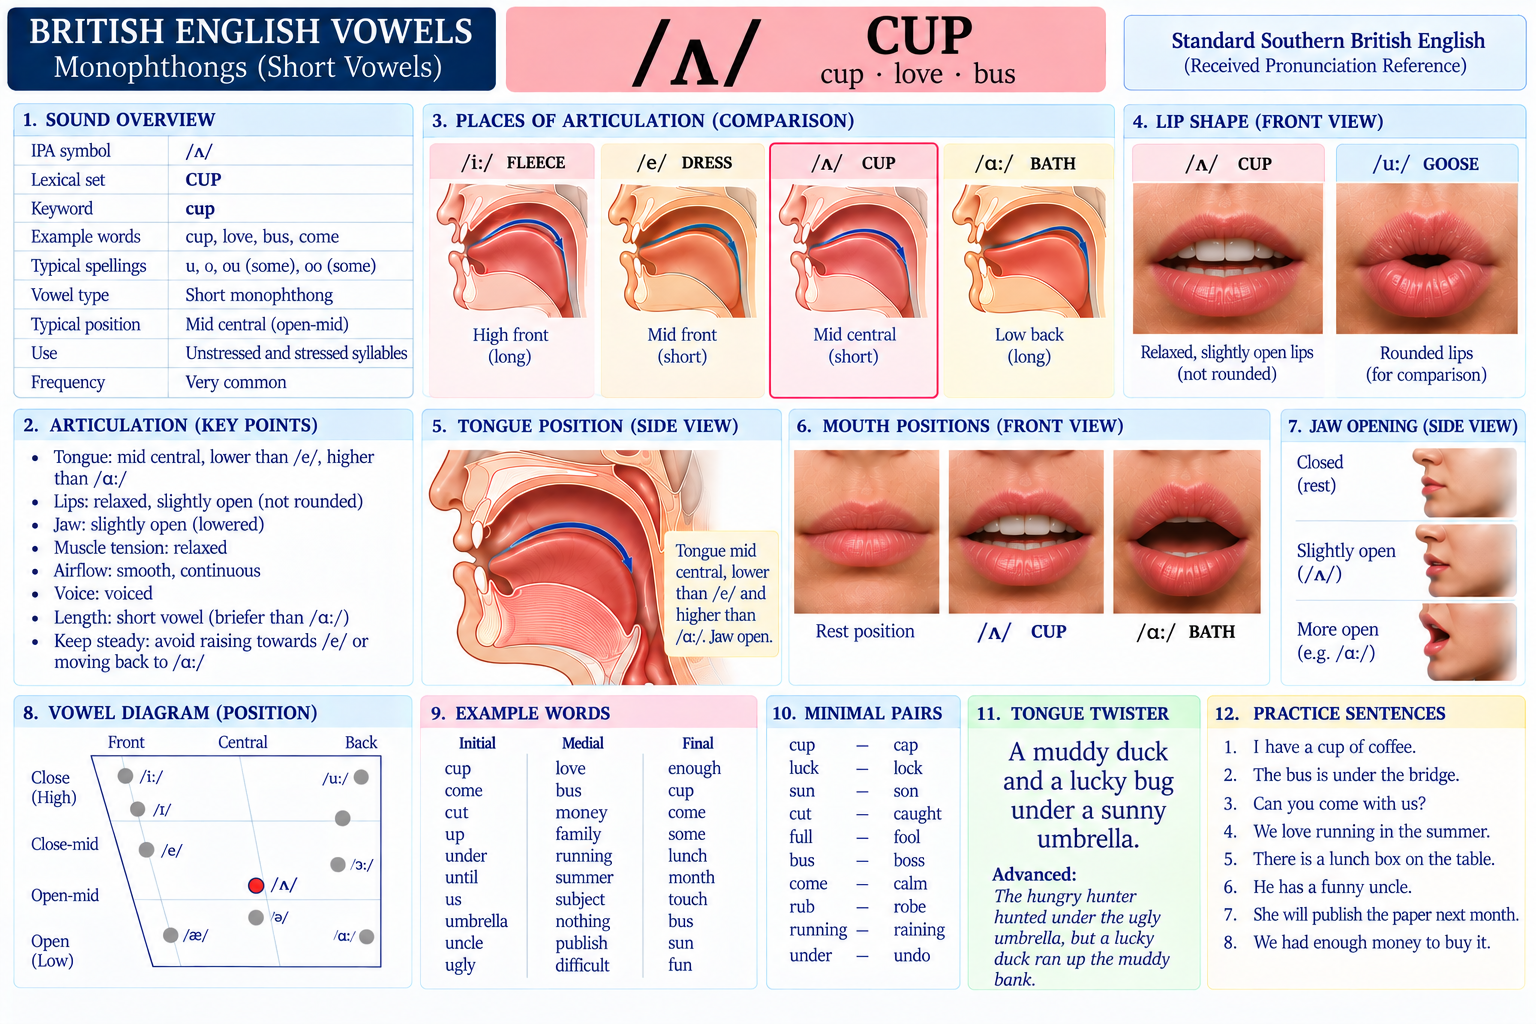
\includegraphics[width=1\linewidth]{images/vowel-u.png}
    \caption{Vowel \ipa{ʌ} construction}
    \label{fig:placeholder}
\end{figure}


\textbf{Lexical anchor:} strut. \textbf{Core examples:} cup, luck, much, money, sun.\par
\textbf{Articulatory target:} Use a central-to-back open-mid target, generally with unrounded lips. Observe tongue-body placement, lip posture and jaw aperture; compare your recording with the reference speaker rather than using spelling as a guide.
\res{FIG-104}{STRUT articulation plate}{Front and sagittal views, highlighted tongue target and lips, vowel-map dot, and comparison with nearest category; SVG and PDF.}
\res{AUD-104}{STRUT native-speaker model}{Isolated target (three repetitions), each example word (slow/natural), minimal-pair contrasts, phrase, sentence and tongue twister; WAV/MP3, transcript and speaker metadata.}
\subsection{Perception and discrimination}
\task{Hear the difference}{Use the companion audio. For ten randomised trials, identify the target vowel or the contrasting vowel. Write your choice and confidence (1--5). Include at least two repeated items to check consistency. No answer can be scored until the audio stimulus list is supplied.}
\res{LST-104}{STRUT discrimination test}{Ten balanced, randomised tokens with answer key, trial order, lexical context and no visible words during listening.}
\subsection{Production ladder}
\begin{enumerate}[label=\arabic*.]
\item Sustain \ipa{ʌ} gently three times; compare with the model.
\item Say each core example in isolation, then embed it in ``I said \emph{[word]} clearly.''
\item Practise the contrasts: cut--cart; luck--lock; hut--hat.
\item Repeat each contrast at slow, conversational and presentation speeds.
\item Record the sentence below and listen for target-vowel consistency.
\end{enumerate}
\textbf{Controlled sentence:} A young consultant discussed the budget.
\subsection{Tongue-twister laboratory}
Say the controlled sentence three times accurately, then twice at natural speed. Mark any vowel that shifts category. Speed is secondary to intelligibility.
\subsection{Reading and transfer}
\task{Mini-reading and spontaneous transfer}{Read the following original prompt aloud, then speak for 30--45 seconds without a script: ``Explain a recent decision, the evidence behind it, and the next action.'' Insert at least three words from this vowel laboratory. Underline them in your transcript and review their pronunciation.}
\res{TXT-104}{STRUT graded reading}{A 100--150-word original passage with 12--20 instances of the target vowel, marked and unmarked versions, vocabulary glosses and comprehension questions.}
\res{REC-104}{STRUT recording worksheet}{Word checklist, contrast accuracy, vowel stability, speaking-rate notes, self-correction and tutor feedback.}

\section{LOT: \ipa{ɒ}}
\label{sec:vowel-05}

\begin{figure}[H]
    \centering
    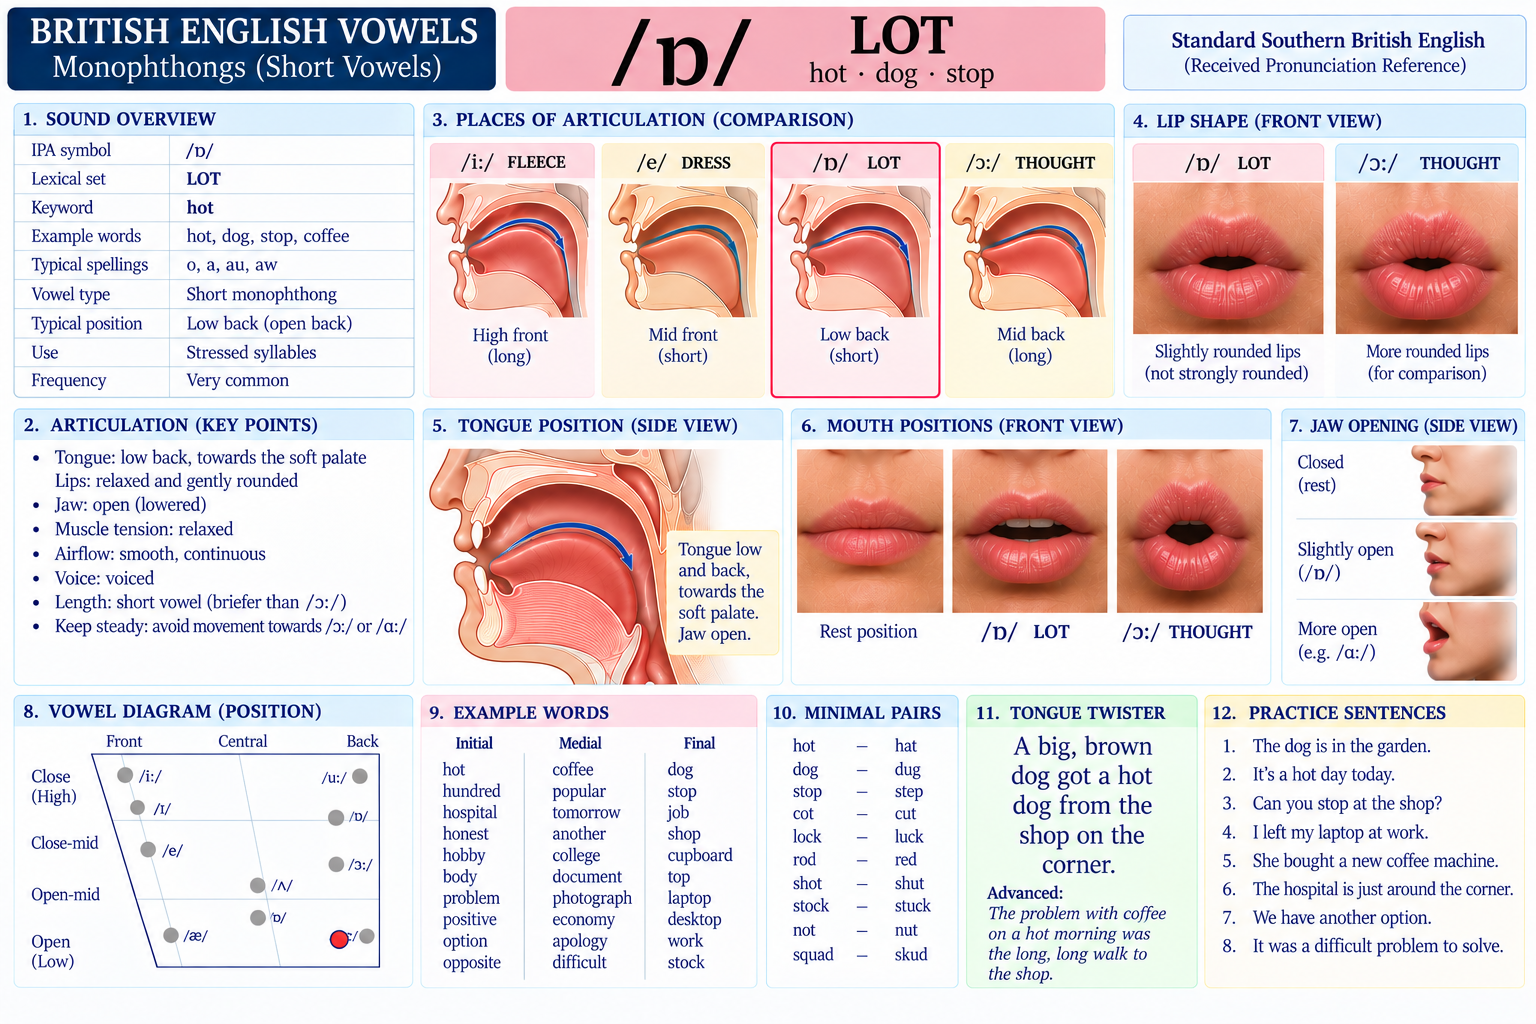
\includegraphics[width=1\linewidth]{images/vowel-a.png}
    \caption{Vowel \ipa{ɒ} construction}
    \label{fig:placeholder}
\end{figure}

\textbf{Lexical anchor:} lot. \textbf{Core examples:} lot, stop, clock, shop, problem.\par
\textbf{Articulatory target:} Aim for a relatively open, back and rounded vowel in the target accent. Observe tongue-body placement, lip posture and jaw aperture; compare your recording with the reference speaker rather than using spelling as a guide.
\res{FIG-105}{LOT articulation plate}{Front and sagittal views, highlighted tongue target and lips, vowel-map dot, and comparison with nearest category; SVG and PDF.}
\res{AUD-105}{LOT native-speaker model}{Isolated target (three repetitions), each example word (slow/natural), minimal-pair contrasts, phrase, sentence and tongue twister; WAV/MP3, transcript and speaker metadata.}
\subsection{Perception and discrimination}
\task{Hear the difference}{Use the companion audio. For ten randomised trials, identify the target vowel or the contrasting vowel. Write your choice and confidence (1--5). Include at least two repeated items to check consistency. No answer can be scored until the audio stimulus list is supplied.}
\res{LST-105}{LOT discrimination test}{Ten balanced, randomised tokens with answer key, trial order, lexical context and no visible words during listening.}
\subsection{Production ladder}
\begin{enumerate}[label=\arabic*.]
\item Sustain \ipa{ɒ} gently three times; compare with the model.
\item Say each core example in isolation, then embed it in ``I said \emph{[word]} clearly.''
\item Practise the contrasts: cot--caught; stock--stalk; not--nought.
\item Repeat each contrast at slow, conversational and presentation speeds.
\item Record the sentence below and listen for target-vowel consistency.
\end{enumerate}
\textbf{Controlled sentence:} The project stopped at the wrong clock.
\subsection{Tongue-twister laboratory}
Say the controlled sentence three times accurately, then twice at natural speed. Mark any vowel that shifts category. Speed is secondary to intelligibility.
\subsection{Reading and transfer}
\task{Mini-reading and spontaneous transfer}{Read the following original prompt aloud, then speak for 30--45 seconds without a script: ``Explain a recent decision, the evidence behind it, and the next action.'' Insert at least three words from this vowel laboratory. Underline them in your transcript and review their pronunciation.}
\res{TXT-105}{LOT graded reading}{A 100--150-word original passage with 12--20 instances of the target vowel, marked and unmarked versions, vocabulary glosses and comprehension questions.}
\res{REC-105}{LOT recording worksheet}{Word checklist, contrast accuracy, vowel stability, speaking-rate notes, self-correction and tutor feedback.}

\section{FOOT: \ipa{ʊ}}
\label{sec:vowel-06}

\begin{figure}[H]
    \centering
    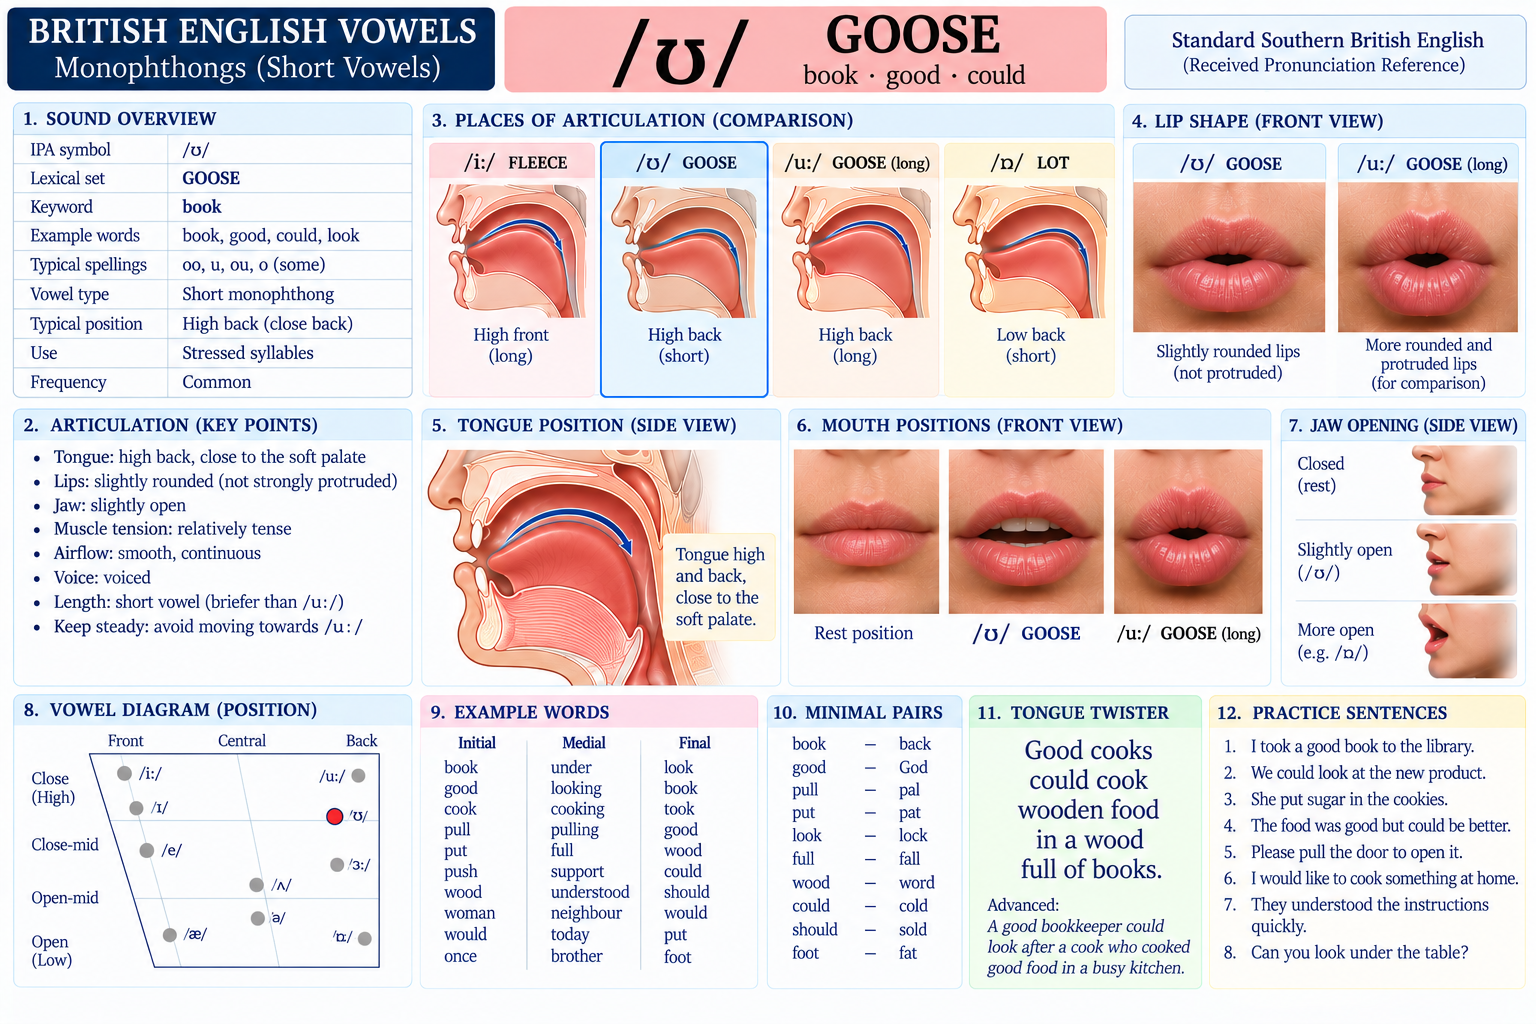
\includegraphics[width=1\linewidth]{images/vowel-uu.png}
    \caption{Vowel \ipa{ʊ} construction}
    \label{fig:placeholder}
\end{figure}

\textbf{Lexical anchor:} foot. \textbf{Core examples:} put, good, book, could, full.\par
\textbf{Articulatory target:} Use a near-high, back-to-central rounded target, distinct from GOOSE. Observe tongue-body placement, lip posture and jaw aperture; compare your recording with the reference speaker rather than using spelling as a guide.
\res{FIG-106}{FOOT articulation plate}{Front and sagittal views, highlighted tongue target and lips, vowel-map dot, and comparison with nearest category; SVG and PDF.}
\res{AUD-106}{FOOT native-speaker model}{Isolated target (three repetitions), each example word (slow/natural), minimal-pair contrasts, phrase, sentence and tongue twister; WAV/MP3, transcript and speaker metadata.}
\subsection{Perception and discrimination}
\task{Hear the difference}{Use the companion audio. For ten randomised trials, identify the target vowel or the contrasting vowel. Write your choice and confidence (1--5). Include at least two repeated items to check consistency. No answer can be scored until the audio stimulus list is supplied.}
\res{LST-106}{FOOT discrimination test}{Ten balanced, randomised tokens with answer key, trial order, lexical context and no visible words during listening.}
\subsection{Production ladder}
\begin{enumerate}[label=\arabic*.]
\item Sustain \ipa{ʊ} gently three times; compare with the model.
\item Say each core example in isolation, then embed it in ``I said \emph{[word]} clearly.''
\item Practise the contrasts: full--fool; pull--pool; look--Luke.
\item Repeat each contrast at slow, conversational and presentation speeds.
\item Record the sentence below and listen for target-vowel consistency.
\end{enumerate}
\textbf{Controlled sentence:} The good cook took a full book.
\subsection{Tongue-twister laboratory}
Say the controlled sentence three times accurately, then twice at natural speed. Mark any vowel that shifts category. Speed is secondary to intelligibility.
\subsection{Reading and transfer}
\task{Mini-reading and spontaneous transfer}{Read the following original prompt aloud, then speak for 30--45 seconds without a script: ``Explain a recent decision, the evidence behind it, and the next action.'' Insert at least three words from this vowel laboratory. Underline them in your transcript and review their pronunciation.}
\res{TXT-106}{FOOT graded reading}{A 100--150-word original passage with 12--20 instances of the target vowel, marked and unmarked versions, vocabulary glosses and comprehension questions.}
\res{REC-106}{FOOT recording worksheet}{Word checklist, contrast accuracy, vowel stability, speaking-rate notes, self-correction and tutor feedback.}

\section{FLEECE: \ipa{iː}}
\label{sec:vowel-07}
\textbf{Lexical anchor:} fleece. \textbf{Core examples:} see, meet, team, leave, machine.\par
\textbf{Articulatory target:} Use a high-front vowel with a stable quality; avoid a strong closing glide. Observe tongue-body placement, lip posture and jaw aperture; compare your recording with the reference speaker rather than using spelling as a guide.
\res{FIG-107}{FLEECE articulation plate}{Front and sagittal views, highlighted tongue target and lips, vowel-map dot, and comparison with nearest category; SVG and PDF.}
\res{AUD-107}{FLEECE native-speaker model}{Isolated target (three repetitions), each example word (slow/natural), minimal-pair contrasts, phrase, sentence and tongue twister; WAV/MP3, transcript and speaker metadata.}
\subsection{Perception and discrimination}
\task{Hear the difference}{Use the companion audio. For ten randomised trials, identify the target vowel or the contrasting vowel. Write your choice and confidence (1--5). Include at least two repeated items to check consistency. No answer can be scored until the audio stimulus list is supplied.}
\res{LST-107}{FLEECE discrimination test}{Ten balanced, randomised tokens with answer key, trial order, lexical context and no visible words during listening.}
\subsection{Production ladder}
\begin{enumerate}[label=\arabic*.]
\item Sustain \ipa{iː} gently three times; compare with the model.
\item Say each core example in isolation, then embed it in ``I said \emph{[word]} clearly.''
\item Practise the contrasts: sheep--ship; seat--sit; reach--rich.
\item Repeat each contrast at slow, conversational and presentation speeds.
\item Record the sentence below and listen for target-vowel consistency.
\end{enumerate}
\textbf{Controlled sentence:} Three keen researchers reviewed the scheme.
\subsection{Tongue-twister laboratory}
Say the controlled sentence three times accurately, then twice at natural speed. Mark any vowel that shifts category. Speed is secondary to intelligibility.
\subsection{Reading and transfer}
\task{Mini-reading and spontaneous transfer}{Read the following original prompt aloud, then speak for 30--45 seconds without a script: ``Explain a recent decision, the evidence behind it, and the next action.'' Insert at least three words from this vowel laboratory. Underline them in your transcript and review their pronunciation.}
\res{TXT-107}{FLEECE graded reading}{A 100--150-word original passage with 12--20 instances of the target vowel, marked and unmarked versions, vocabulary glosses and comprehension questions.}
\res{REC-107}{FLEECE recording worksheet}{Word checklist, contrast accuracy, vowel stability, speaking-rate notes, self-correction and tutor feedback.}

\section{GOOSE: \ipa{uː}}
\label{sec:vowel-08}
\textbf{Lexical anchor:} goose. \textbf{Core examples:} food, blue, move, group, student.\par
\textbf{Articulatory target:} Use a high vowel with rounding; many modern speakers have a noticeably fronted tongue position. Observe tongue-body placement, lip posture and jaw aperture; compare your recording with the reference speaker rather than using spelling as a guide.
\res{FIG-108}{GOOSE articulation plate}{Front and sagittal views, highlighted tongue target and lips, vowel-map dot, and comparison with nearest category; SVG and PDF.}
\res{AUD-108}{GOOSE native-speaker model}{Isolated target (three repetitions), each example word (slow/natural), minimal-pair contrasts, phrase, sentence and tongue twister; WAV/MP3, transcript and speaker metadata.}
\subsection{Perception and discrimination}
\task{Hear the difference}{Use the companion audio. For ten randomised trials, identify the target vowel or the contrasting vowel. Write your choice and confidence (1--5). Include at least two repeated items to check consistency. No answer can be scored until the audio stimulus list is supplied.}
\res{LST-108}{GOOSE discrimination test}{Ten balanced, randomised tokens with answer key, trial order, lexical context and no visible words during listening.}
\subsection{Production ladder}
\begin{enumerate}[label=\arabic*.]
\item Sustain \ipa{uː} gently three times; compare with the model.
\item Say each core example in isolation, then embed it in ``I said \emph{[word]} clearly.''
\item Practise the contrasts: fool--full; pool--pull; Luke--look.
\item Repeat each contrast at slow, conversational and presentation speeds.
\item Record the sentence below and listen for target-vowel consistency.
\end{enumerate}
\textbf{Controlled sentence:} Two students moved the blue tools.
\subsection{Tongue-twister laboratory}
Say the controlled sentence three times accurately, then twice at natural speed. Mark any vowel that shifts category. Speed is secondary to intelligibility.
\subsection{Reading and transfer}
\task{Mini-reading and spontaneous transfer}{Read the following original prompt aloud, then speak for 30--45 seconds without a script: ``Explain a recent decision, the evidence behind it, and the next action.'' Insert at least three words from this vowel laboratory. Underline them in your transcript and review their pronunciation.}
\res{TXT-108}{GOOSE graded reading}{A 100--150-word original passage with 12--20 instances of the target vowel, marked and unmarked versions, vocabulary glosses and comprehension questions.}
\res{REC-108}{GOOSE recording worksheet}{Word checklist, contrast accuracy, vowel stability, speaking-rate notes, self-correction and tutor feedback.}

\section{PALM: \ipa{ɑː}}
\label{sec:vowel-09}
\textbf{Lexical anchor:} palm. \textbf{Core examples:} father, calm, start, hard, class.\par
\textbf{Articulatory target:} Use an open back unrounded target; note non-rhotic spelling in start and hard. Observe tongue-body placement, lip posture and jaw aperture; compare your recording with the reference speaker rather than using spelling as a guide.
\res{FIG-109}{PALM articulation plate}{Front and sagittal views, highlighted tongue target and lips, vowel-map dot, and comparison with nearest category; SVG and PDF.}
\res{AUD-109}{PALM native-speaker model}{Isolated target (three repetitions), each example word (slow/natural), minimal-pair contrasts, phrase, sentence and tongue twister; WAV/MP3, transcript and speaker metadata.}
\subsection{Perception and discrimination}
\task{Hear the difference}{Use the companion audio. For ten randomised trials, identify the target vowel or the contrasting vowel. Write your choice and confidence (1--5). Include at least two repeated items to check consistency. No answer can be scored until the audio stimulus list is supplied.}
\res{LST-109}{PALM discrimination test}{Ten balanced, randomised tokens with answer key, trial order, lexical context and no visible words during listening.}
\subsection{Production ladder}
\begin{enumerate}[label=\arabic*.]
\item Sustain \ipa{ɑː} gently three times; compare with the model.
\item Say each core example in isolation, then embed it in ``I said \emph{[word]} clearly.''
\item Practise the contrasts: cart--cut; heart--hut; bard--bad.
\item Repeat each contrast at slow, conversational and presentation speeds.
\item Record the sentence below and listen for target-vowel consistency.
\end{enumerate}
\textbf{Controlled sentence:} The department started a large task.
\subsection{Tongue-twister laboratory}
Say the controlled sentence three times accurately, then twice at natural speed. Mark any vowel that shifts category. Speed is secondary to intelligibility.
\subsection{Reading and transfer}
\task{Mini-reading and spontaneous transfer}{Read the following original prompt aloud, then speak for 30--45 seconds without a script: ``Explain a recent decision, the evidence behind it, and the next action.'' Insert at least three words from this vowel laboratory. Underline them in your transcript and review their pronunciation.}
\res{TXT-109}{PALM graded reading}{A 100--150-word original passage with 12--20 instances of the target vowel, marked and unmarked versions, vocabulary glosses and comprehension questions.}
\res{REC-109}{PALM recording worksheet}{Word checklist, contrast accuracy, vowel stability, speaking-rate notes, self-correction and tutor feedback.}

\section{THOUGHT: \ipa{ɔː}}
\label{sec:vowel-10}
\textbf{Lexical anchor:} thought. \textbf{Core examples:} thought, law, talk, caught, order.\par
\textbf{Articulatory target:} Use a mid-open back rounded target; non-rhotic spelling may contain r. Observe tongue-body placement, lip posture and jaw aperture; compare your recording with the reference speaker rather than using spelling as a guide.
\res{FIG-110}{THOUGHT articulation plate}{Front and sagittal views, highlighted tongue target and lips, vowel-map dot, and comparison with nearest category; SVG and PDF.}
\res{AUD-110}{THOUGHT native-speaker model}{Isolated target (three repetitions), each example word (slow/natural), minimal-pair contrasts, phrase, sentence and tongue twister; WAV/MP3, transcript and speaker metadata.}
\subsection{Perception and discrimination}
\task{Hear the difference}{Use the companion audio. For ten randomised trials, identify the target vowel or the contrasting vowel. Write your choice and confidence (1--5). Include at least two repeated items to check consistency. No answer can be scored until the audio stimulus list is supplied.}
\res{LST-110}{THOUGHT discrimination test}{Ten balanced, randomised tokens with answer key, trial order, lexical context and no visible words during listening.}
\subsection{Production ladder}
\begin{enumerate}[label=\arabic*.]
\item Sustain \ipa{ɔː} gently three times; compare with the model.
\item Say each core example in isolation, then embed it in ``I said \emph{[word]} clearly.''
\item Practise the contrasts: caught--cot; port--pot; dawn--Don.
\item Repeat each contrast at slow, conversational and presentation speeds.
\item Record the sentence below and listen for target-vowel consistency.
\end{enumerate}
\textbf{Controlled sentence:} The board thought the report was important.
\subsection{Tongue-twister laboratory}
Say the controlled sentence three times accurately, then twice at natural speed. Mark any vowel that shifts category. Speed is secondary to intelligibility.
\subsection{Reading and transfer}
\task{Mini-reading and spontaneous transfer}{Read the following original prompt aloud, then speak for 30--45 seconds without a script: ``Explain a recent decision, the evidence behind it, and the next action.'' Insert at least three words from this vowel laboratory. Underline them in your transcript and review their pronunciation.}
\res{TXT-110}{THOUGHT graded reading}{A 100--150-word original passage with 12--20 instances of the target vowel, marked and unmarked versions, vocabulary glosses and comprehension questions.}
\res{REC-110}{THOUGHT recording worksheet}{Word checklist, contrast accuracy, vowel stability, speaking-rate notes, self-correction and tutor feedback.}

\section{NURSE: \ipa{ɜː}}
\label{sec:vowel-11}
\textbf{Lexical anchor:} nurse. \textbf{Core examples:} bird, word, work, learn, first.\par
\textbf{Articulatory target:} Use a long central vowel without pronouncing postvocalic r in isolated non-rhotic words. Observe tongue-body placement, lip posture and jaw aperture; compare your recording with the reference speaker rather than using spelling as a guide.
\res{FIG-111}{NURSE articulation plate}{Front and sagittal views, highlighted tongue target and lips, vowel-map dot, and comparison with nearest category; SVG and PDF.}
\res{AUD-111}{NURSE native-speaker model}{Isolated target (three repetitions), each example word (slow/natural), minimal-pair contrasts, phrase, sentence and tongue twister; WAV/MP3, transcript and speaker metadata.}
\subsection{Perception and discrimination}
\task{Hear the difference}{Use the companion audio. For ten randomised trials, identify the target vowel or the contrasting vowel. Write your choice and confidence (1--5). Include at least two repeated items to check consistency. No answer can be scored until the audio stimulus list is supplied.}
\res{LST-111}{NURSE discrimination test}{Ten balanced, randomised tokens with answer key, trial order, lexical context and no visible words during listening.}
\subsection{Production ladder}
\begin{enumerate}[label=\arabic*.]
\item Sustain \ipa{ɜː} gently three times; compare with the model.
\item Say each core example in isolation, then embed it in ``I said \emph{[word]} clearly.''
\item Practise the contrasts: bird--bud; word--wood; hurt--hut.
\item Repeat each contrast at slow, conversational and presentation speeds.
\item Record the sentence below and listen for target-vowel consistency.
\end{enumerate}
\textbf{Controlled sentence:} The first researcher learnt the terms.
\subsection{Tongue-twister laboratory}
Say the controlled sentence three times accurately, then twice at natural speed. Mark any vowel that shifts category. Speed is secondary to intelligibility.
\subsection{Reading and transfer}
\task{Mini-reading and spontaneous transfer}{Read the following original prompt aloud, then speak for 30--45 seconds without a script: ``Explain a recent decision, the evidence behind it, and the next action.'' Insert at least three words from this vowel laboratory. Underline them in your transcript and review their pronunciation.}
\res{TXT-111}{NURSE graded reading}{A 100--150-word original passage with 12--20 instances of the target vowel, marked and unmarked versions, vocabulary glosses and comprehension questions.}
\res{REC-111}{NURSE recording worksheet}{Word checklist, contrast accuracy, vowel stability, speaking-rate notes, self-correction and tutor feedback.}

\section{FACE: \ipa{eɪ}}
\label{sec:vowel-12}
\textbf{Lexical anchor:} face. \textbf{Core examples:} day, make, train, eight, data.\par
\textbf{Articulatory target:} Begin around mid-front and glide towards a higher front position. Observe tongue-body placement, lip posture and jaw aperture; compare your recording with the reference speaker rather than using spelling as a guide.
\res{FIG-112}{FACE articulation plate}{Front and sagittal views, highlighted tongue target and lips, vowel-map dot, and comparison with nearest category; SVG and PDF.}
\res{AUD-112}{FACE native-speaker model}{Isolated target (three repetitions), each example word (slow/natural), minimal-pair contrasts, phrase, sentence and tongue twister; WAV/MP3, transcript and speaker metadata.}
\subsection{Perception and discrimination}
\task{Hear the difference}{Use the companion audio. For ten randomised trials, identify the target vowel or the contrasting vowel. Write your choice and confidence (1--5). Include at least two repeated items to check consistency. No answer can be scored until the audio stimulus list is supplied.}
\res{LST-112}{FACE discrimination test}{Ten balanced, randomised tokens with answer key, trial order, lexical context and no visible words during listening.}
\subsection{Production ladder}
\begin{enumerate}[label=\arabic*.]
\item Sustain \ipa{eɪ} gently three times; compare with the model.
\item Say each core example in isolation, then embed it in ``I said \emph{[word]} clearly.''
\item Practise the contrasts: late--light; wait--white.
\item Repeat each contrast at slow, conversational and presentation speeds.
\item Record the sentence below and listen for target-vowel consistency.
\end{enumerate}
\textbf{Controlled sentence:} They made a detailed case today.
\subsection{Tongue-twister laboratory}
Say the controlled sentence three times accurately, then twice at natural speed. Mark any vowel that shifts category. Speed is secondary to intelligibility.
\subsection{Reading and transfer}
\task{Mini-reading and spontaneous transfer}{Read the following original prompt aloud, then speak for 30--45 seconds without a script: ``Explain a recent decision, the evidence behind it, and the next action.'' Insert at least three words from this vowel laboratory. Underline them in your transcript and review their pronunciation.}
\res{TXT-112}{FACE graded reading}{A 100--150-word original passage with 12--20 instances of the target vowel, marked and unmarked versions, vocabulary glosses and comprehension questions.}
\res{REC-112}{FACE recording worksheet}{Word checklist, contrast accuracy, vowel stability, speaking-rate notes, self-correction and tutor feedback.}

\section{PRICE: \ipa{aɪ}}
\label{sec:vowel-13}
\textbf{Lexical anchor:} price. \textbf{Core examples:} time, high, find, science, trial.\par
\textbf{Articulatory target:} Begin open and glide towards a near-high front position. Observe tongue-body placement, lip posture and jaw aperture; compare your recording with the reference speaker rather than using spelling as a guide.
\res{FIG-113}{PRICE articulation plate}{Front and sagittal views, highlighted tongue target and lips, vowel-map dot, and comparison with nearest category; SVG and PDF.}
\res{AUD-113}{PRICE native-speaker model}{Isolated target (three repetitions), each example word (slow/natural), minimal-pair contrasts, phrase, sentence and tongue twister; WAV/MP3, transcript and speaker metadata.}
\subsection{Perception and discrimination}
\task{Hear the difference}{Use the companion audio. For ten randomised trials, identify the target vowel or the contrasting vowel. Write your choice and confidence (1--5). Include at least two repeated items to check consistency. No answer can be scored until the audio stimulus list is supplied.}
\res{LST-113}{PRICE discrimination test}{Ten balanced, randomised tokens with answer key, trial order, lexical context and no visible words during listening.}
\subsection{Production ladder}
\begin{enumerate}[label=\arabic*.]
\item Sustain \ipa{aɪ} gently three times; compare with the model.
\item Say each core example in isolation, then embed it in ``I said \emph{[word]} clearly.''
\item Practise the contrasts: price--press; line--lane.
\item Repeat each contrast at slow, conversational and presentation speeds.
\item Record the sentence below and listen for target-vowel consistency.
\end{enumerate}
\textbf{Controlled sentence:} I will finalise the findings by Friday.
\subsection{Tongue-twister laboratory}
Say the controlled sentence three times accurately, then twice at natural speed. Mark any vowel that shifts category. Speed is secondary to intelligibility.
\subsection{Reading and transfer}
\task{Mini-reading and spontaneous transfer}{Read the following original prompt aloud, then speak for 30--45 seconds without a script: ``Explain a recent decision, the evidence behind it, and the next action.'' Insert at least three words from this vowel laboratory. Underline them in your transcript and review their pronunciation.}
\res{TXT-113}{PRICE graded reading}{A 100--150-word original passage with 12--20 instances of the target vowel, marked and unmarked versions, vocabulary glosses and comprehension questions.}
\res{REC-113}{PRICE recording worksheet}{Word checklist, contrast accuracy, vowel stability, speaking-rate notes, self-correction and tutor feedback.}

\section{CHOICE: \ipa{ɔɪ}}
\label{sec:vowel-14}
\textbf{Lexical anchor:} choice. \textbf{Core examples:} choice, point, voice, join, noise.\par
\textbf{Articulatory target:} Begin rounded and back, then glide towards the front. Observe tongue-body placement, lip posture and jaw aperture; compare your recording with the reference speaker rather than using spelling as a guide.
\res{FIG-114}{CHOICE articulation plate}{Front and sagittal views, highlighted tongue target and lips, vowel-map dot, and comparison with nearest category; SVG and PDF.}
\res{AUD-114}{CHOICE native-speaker model}{Isolated target (three repetitions), each example word (slow/natural), minimal-pair contrasts, phrase, sentence and tongue twister; WAV/MP3, transcript and speaker metadata.}
\subsection{Perception and discrimination}
\task{Hear the difference}{Use the companion audio. For ten randomised trials, identify the target vowel or the contrasting vowel. Write your choice and confidence (1--5). Include at least two repeated items to check consistency. No answer can be scored until the audio stimulus list is supplied.}
\res{LST-114}{CHOICE discrimination test}{Ten balanced, randomised tokens with answer key, trial order, lexical context and no visible words during listening.}
\subsection{Production ladder}
\begin{enumerate}[label=\arabic*.]
\item Sustain \ipa{ɔɪ} gently three times; compare with the model.
\item Say each core example in isolation, then embed it in ``I said \emph{[word]} clearly.''
\item Practise the contrasts: boy--buy; toy--tie.
\item Repeat each contrast at slow, conversational and presentation speeds.
\item Record the sentence below and listen for target-vowel consistency.
\end{enumerate}
\textbf{Controlled sentence:} The joint choice avoided the noise.
\subsection{Tongue-twister laboratory}
Say the controlled sentence three times accurately, then twice at natural speed. Mark any vowel that shifts category. Speed is secondary to intelligibility.
\subsection{Reading and transfer}
\task{Mini-reading and spontaneous transfer}{Read the following original prompt aloud, then speak for 30--45 seconds without a script: ``Explain a recent decision, the evidence behind it, and the next action.'' Insert at least three words from this vowel laboratory. Underline them in your transcript and review their pronunciation.}
\res{TXT-114}{CHOICE graded reading}{A 100--150-word original passage with 12--20 instances of the target vowel, marked and unmarked versions, vocabulary glosses and comprehension questions.}
\res{REC-114}{CHOICE recording worksheet}{Word checklist, contrast accuracy, vowel stability, speaking-rate notes, self-correction and tutor feedback.}

\section{GOAT: \ipa{əʊ}}
\label{sec:vowel-15}
\textbf{Lexical anchor:} goat. \textbf{Core examples:} go, home, show, road, approach.\par
\textbf{Articulatory target:} Start centrally in the traditional model and glide towards a higher rounded position; modern onsets vary. Observe tongue-body placement, lip posture and jaw aperture; compare your recording with the reference speaker rather than using spelling as a guide.
\res{FIG-115}{GOAT articulation plate}{Front and sagittal views, highlighted tongue target and lips, vowel-map dot, and comparison with nearest category; SVG and PDF.}
\res{AUD-115}{GOAT native-speaker model}{Isolated target (three repetitions), each example word (slow/natural), minimal-pair contrasts, phrase, sentence and tongue twister; WAV/MP3, transcript and speaker metadata.}
\subsection{Perception and discrimination}
\task{Hear the difference}{Use the companion audio. For ten randomised trials, identify the target vowel or the contrasting vowel. Write your choice and confidence (1--5). Include at least two repeated items to check consistency. No answer can be scored until the audio stimulus list is supplied.}
\res{LST-115}{GOAT discrimination test}{Ten balanced, randomised tokens with answer key, trial order, lexical context and no visible words during listening.}
\subsection{Production ladder}
\begin{enumerate}[label=\arabic*.]
\item Sustain \ipa{əʊ} gently three times; compare with the model.
\item Say each core example in isolation, then embed it in ``I said \emph{[word]} clearly.''
\item Practise the contrasts: coat--kite; low--lie.
\item Repeat each contrast at slow, conversational and presentation speeds.
\item Record the sentence below and listen for target-vowel consistency.
\end{enumerate}
\textbf{Controlled sentence:} We showed the whole approach.
\subsection{Tongue-twister laboratory}
Say the controlled sentence three times accurately, then twice at natural speed. Mark any vowel that shifts category. Speed is secondary to intelligibility.
\subsection{Reading and transfer}
\task{Mini-reading and spontaneous transfer}{Read the following original prompt aloud, then speak for 30--45 seconds without a script: ``Explain a recent decision, the evidence behind it, and the next action.'' Insert at least three words from this vowel laboratory. Underline them in your transcript and review their pronunciation.}
\res{TXT-115}{GOAT graded reading}{A 100--150-word original passage with 12--20 instances of the target vowel, marked and unmarked versions, vocabulary glosses and comprehension questions.}
\res{REC-115}{GOAT recording worksheet}{Word checklist, contrast accuracy, vowel stability, speaking-rate notes, self-correction and tutor feedback.}

\section{MOUTH: \ipa{aʊ}}
\label{sec:vowel-16}
\textbf{Lexical anchor:} mouth. \textbf{Core examples:} now, house, sound, about, outcome.\par
\textbf{Articulatory target:} Start open and move towards a high rounded target; keep a genuine glide. Observe tongue-body placement, lip posture and jaw aperture; compare your recording with the reference speaker rather than using spelling as a guide.
\res{FIG-116}{MOUTH articulation plate}{Front and sagittal views, highlighted tongue target and lips, vowel-map dot, and comparison with nearest category; SVG and PDF.}
\res{AUD-116}{MOUTH native-speaker model}{Isolated target (three repetitions), each example word (slow/natural), minimal-pair contrasts, phrase, sentence and tongue twister; WAV/MP3, transcript and speaker metadata.}
\subsection{Perception and discrimination}
\task{Hear the difference}{Use the companion audio. For ten randomised trials, identify the target vowel or the contrasting vowel. Write your choice and confidence (1--5). Include at least two repeated items to check consistency. No answer can be scored until the audio stimulus list is supplied.}
\res{LST-116}{MOUTH discrimination test}{Ten balanced, randomised tokens with answer key, trial order, lexical context and no visible words during listening.}
\subsection{Production ladder}
\begin{enumerate}[label=\arabic*.]
\item Sustain \ipa{aʊ} gently three times; compare with the model.
\item Say each core example in isolation, then embed it in ``I said \emph{[word]} clearly.''
\item Practise the contrasts: loud--lied; town--time.
\item Repeat each contrast at slow, conversational and presentation speeds.
\item Record the sentence below and listen for target-vowel consistency.
\end{enumerate}
\textbf{Controlled sentence:} Now outline the outcome aloud.
\subsection{Tongue-twister laboratory}
Say the controlled sentence three times accurately, then twice at natural speed. Mark any vowel that shifts category. Speed is secondary to intelligibility.
\subsection{Reading and transfer}
\task{Mini-reading and spontaneous transfer}{Read the following original prompt aloud, then speak for 30--45 seconds without a script: ``Explain a recent decision, the evidence behind it, and the next action.'' Insert at least three words from this vowel laboratory. Underline them in your transcript and review their pronunciation.}
\res{TXT-116}{MOUTH graded reading}{A 100--150-word original passage with 12--20 instances of the target vowel, marked and unmarked versions, vocabulary glosses and comprehension questions.}
\res{REC-116}{MOUTH recording worksheet}{Word checklist, contrast accuracy, vowel stability, speaking-rate notes, self-correction and tutor feedback.}

\section{NEAR: \ipa{ɪə}}
\label{sec:vowel-17}
\textbf{Lexical anchor:} near. \textbf{Core examples:} near, here, clear, idea, serious.\par
\textbf{Articulatory target:} Traditional centring diphthong; many current speakers use a more monophthongal realisation. Observe tongue-body placement, lip posture and jaw aperture; compare your recording with the reference speaker rather than using spelling as a guide.
\res{FIG-117}{NEAR articulation plate}{Front and sagittal views, highlighted tongue target and lips, vowel-map dot, and comparison with nearest category; SVG and PDF.}
\res{AUD-117}{NEAR native-speaker model}{Isolated target (three repetitions), each example word (slow/natural), minimal-pair contrasts, phrase, sentence and tongue twister; WAV/MP3, transcript and speaker metadata.}
\subsection{Perception and discrimination}
\task{Hear the difference}{Use the companion audio. For ten randomised trials, identify the target vowel or the contrasting vowel. Write your choice and confidence (1--5). Include at least two repeated items to check consistency. No answer can be scored until the audio stimulus list is supplied.}
\res{LST-117}{NEAR discrimination test}{Ten balanced, randomised tokens with answer key, trial order, lexical context and no visible words during listening.}
\subsection{Production ladder}
\begin{enumerate}[label=\arabic*.]
\item Sustain \ipa{ɪə} gently three times; compare with the model.
\item Say each core example in isolation, then embed it in ``I said \emph{[word]} clearly.''
\item Practise the contrasts: near--narrow (non-minimal contrast).
\item Repeat each contrast at slow, conversational and presentation speeds.
\item Record the sentence below and listen for target-vowel consistency.
\end{enumerate}
\textbf{Controlled sentence:} The engineer gave a clear idea.
\subsection{Tongue-twister laboratory}
Say the controlled sentence three times accurately, then twice at natural speed. Mark any vowel that shifts category. Speed is secondary to intelligibility.
\subsection{Reading and transfer}
\task{Mini-reading and spontaneous transfer}{Read the following original prompt aloud, then speak for 30--45 seconds without a script: ``Explain a recent decision, the evidence behind it, and the next action.'' Insert at least three words from this vowel laboratory. Underline them in your transcript and review their pronunciation.}
\res{TXT-117}{NEAR graded reading}{A 100--150-word original passage with 12--20 instances of the target vowel, marked and unmarked versions, vocabulary glosses and comprehension questions.}
\res{REC-117}{NEAR recording worksheet}{Word checklist, contrast accuracy, vowel stability, speaking-rate notes, self-correction and tutor feedback.}

\section{SQUARE: \ipa{eə}}
\label{sec:vowel-18}
\textbf{Lexical anchor:} square. \textbf{Core examples:} care, fair, square, share, various.\par
\textbf{Articulatory target:} Traditional centring diphthong; modern speakers may use a long monophthong. Observe tongue-body placement, lip posture and jaw aperture; compare your recording with the reference speaker rather than using spelling as a guide.
\res{FIG-118}{SQUARE articulation plate}{Front and sagittal views, highlighted tongue target and lips, vowel-map dot, and comparison with nearest category; SVG and PDF.}
\res{AUD-118}{SQUARE native-speaker model}{Isolated target (three repetitions), each example word (slow/natural), minimal-pair contrasts, phrase, sentence and tongue twister; WAV/MP3, transcript and speaker metadata.}
\subsection{Perception and discrimination}
\task{Hear the difference}{Use the companion audio. For ten randomised trials, identify the target vowel or the contrasting vowel. Write your choice and confidence (1--5). Include at least two repeated items to check consistency. No answer can be scored until the audio stimulus list is supplied.}
\res{LST-118}{SQUARE discrimination test}{Ten balanced, randomised tokens with answer key, trial order, lexical context and no visible words during listening.}
\subsection{Production ladder}
\begin{enumerate}[label=\arabic*.]
\item Sustain \ipa{eə} gently three times; compare with the model.
\item Say each core example in isolation, then embed it in ``I said \emph{[word]} clearly.''
\item Practise the contrasts: fair--fear.
\item Repeat each contrast at slow, conversational and presentation speeds.
\item Record the sentence below and listen for target-vowel consistency.
\end{enumerate}
\textbf{Controlled sentence:} Please share a fair comparison.
\subsection{Tongue-twister laboratory}
Say the controlled sentence three times accurately, then twice at natural speed. Mark any vowel that shifts category. Speed is secondary to intelligibility.
\subsection{Reading and transfer}
\task{Mini-reading and spontaneous transfer}{Read the following original prompt aloud, then speak for 30--45 seconds without a script: ``Explain a recent decision, the evidence behind it, and the next action.'' Insert at least three words from this vowel laboratory. Underline them in your transcript and review their pronunciation.}
\res{TXT-118}{SQUARE graded reading}{A 100--150-word original passage with 12--20 instances of the target vowel, marked and unmarked versions, vocabulary glosses and comprehension questions.}
\res{REC-118}{SQUARE recording worksheet}{Word checklist, contrast accuracy, vowel stability, speaking-rate notes, self-correction and tutor feedback.}

\section{CURE: \ipa{ʊə}}
\label{sec:vowel-19}
\textbf{Lexical anchor:} cure. \textbf{Core examples:} cure, tourist, pure, secure.\par
\textbf{Articulatory target:} This category is unstable in contemporary SSBE; distinguish lexical and speaker-specific pronunciations. Observe tongue-body placement, lip posture and jaw aperture; compare your recording with the reference speaker rather than using spelling as a guide.
\res{FIG-119}{CURE articulation plate}{Front and sagittal views, highlighted tongue target and lips, vowel-map dot, and comparison with nearest category; SVG and PDF.}
\res{AUD-119}{CURE native-speaker model}{Isolated target (three repetitions), each example word (slow/natural), minimal-pair contrasts, phrase, sentence and tongue twister; WAV/MP3, transcript and speaker metadata.}
\subsection{Perception and discrimination}
\task{Hear the difference}{Use the companion audio. For ten randomised trials, identify the target vowel or the contrasting vowel. Write your choice and confidence (1--5). Include at least two repeated items to check consistency. No answer can be scored until the audio stimulus list is supplied.}
\res{LST-119}{CURE discrimination test}{Ten balanced, randomised tokens with answer key, trial order, lexical context and no visible words during listening.}
\subsection{Production ladder}
\begin{enumerate}[label=\arabic*.]
\item Sustain \ipa{ʊə} gently three times; compare with the model.
\item Say each core example in isolation, then embed it in ``I said \emph{[word]} clearly.''
\item Practise the contrasts: poor--paw (accent-dependent).
\item Repeat each contrast at slow, conversational and presentation speeds.
\item Record the sentence below and listen for target-vowel consistency.
\end{enumerate}
\textbf{Controlled sentence:} The tourist was unsure about the cure.
\subsection{Tongue-twister laboratory}
Say the controlled sentence three times accurately, then twice at natural speed. Mark any vowel that shifts category. Speed is secondary to intelligibility.
\subsection{Reading and transfer}
\task{Mini-reading and spontaneous transfer}{Read the following original prompt aloud, then speak for 30--45 seconds without a script: ``Explain a recent decision, the evidence behind it, and the next action.'' Insert at least three words from this vowel laboratory. Underline them in your transcript and review their pronunciation.}
\res{TXT-119}{CURE graded reading}{A 100--150-word original passage with 12--20 instances of the target vowel, marked and unmarked versions, vocabulary glosses and comprehension questions.}
\res{REC-119}{CURE recording worksheet}{Word checklist, contrast accuracy, vowel stability, speaking-rate notes, self-correction and tutor feedback.}
\section{Schwa and weak-vowel systems}
The schwa \ipa{ə} is a central vowel frequently found in unstressed syllables: \emph{about} /əˈbaʊt/, \emph{teacher} /ˈtiːtʃə/ in non-rhotic speech. Unstressed vowels also include weak /ɪ/ and word-final /i/ in many descriptions. Vowel reduction is not simply speaking quickly: it reflects lexical stress, grammatical function and prosodic structure.
\begin{longtable}{lll}
\toprule Word & Strong form (illustrative) & Weak form (illustrative)\\\midrule\endhead
can & /kæn/ & /kən/\\
to & /tuː/ & /tə/\\
for & /fɔː/ & /fə/\\
and & /ænd/ & /ən/\\
of & /ɒv/ & /əv/\\
\bottomrule\end{longtable}
\noindent Weak forms are context-dependent; strong forms can occur under contrastive stress or at certain prosodic boundaries. The table is not a rule to reduce every occurrence.
\task{Mark the reductions}{Read: ``I can send the report to the team, and we can discuss it at the meeting.'' Underline grammatical words that may have weak forms in neutral fluent speech. Record one careful version and one natural version; explain the differences.}
\res{AUD-300}{Strong/weak form contrast pack}{Twenty matched sentences, two rates, phrase-level stress annotation, transcripts and answer key.}
\res{FIG-300}{Stress and reduction diagram}{Prominence peaks, unstressed syllables, and schwa locations aligned to an authentic spoken sentence.}
\section{Vowels in connected speech}
\subsection{Rhythm and prominence}
English rhythm is influenced by prominence and reductions, not by an absolute rule that stressed syllables occur at equal intervals. Mark content words, focus words and reduced grammatical words in short utterances.
\subsection{Non-rhoticity, linking and intrusive r}
In the target accent, postvocalic /r/ is generally absent before consonants or pauses (\emph{car}, \emph{hard}), but an /r/ may surface before a following vowel (\emph{far away}); an intrusive /r/ may also occur in sequences such as \emph{law and order}. Usage varies by speaker and register.
\res{AUD-301}{Connected-speech contrasts}{Careful and natural recordings: far away, car park, law and order, here it is, and other controlled contexts.}
\subsection{Coarticulation and speech rate}
Vowel targets shift in fluent speech under the influence of neighbouring sounds. Practise maintaining intelligible contrasts without attempting to make every vowel sound identical to its isolated dictionary form.
\task{Meeting simulation}{Explain a project delay in 90 seconds. Include a problem, its cause, two options and a recommendation. Replay your recording and mark prominent words, schwas, and any vowel contrasts that collapsed.}
\section{Listening and shadowing laboratory}
\begin{enumerate}[label=\arabic*.]
\item Listen without a transcript and identify the topic.
\item Listen again and transcribe a short excerpt.
\item Compare your transcript with the official version and mark vowel-based misunderstandings.
\item Shadow in 3--5-second chunks, imitating prominence and reductions.
\item Record an independent retelling; assess intelligibility and target-vowel stability.
\end{enumerate}
\res{AUD-400}{Graded listening corpus}{Eight recordings: everyday conversation, directions, telephone exchange, workplace update, technical meeting, research summary, short lecture and natural-speed interview; each with clean transcript and timestamps.}
\res{VID-400}{Visible-speech reference}{Short native-speaker video showing lips and jaw during representative vowels and diphthongs; captions and normal/slow playback.}
\section{Professional and academic readings}
\subsection{Reading A: Explaining a data pipeline}
``Our data pipeline receives records from several sources. First, the system checks the file format and validates the required fields. Next, it transforms the records into a consistent structure. Finally, the team reviews the results and reports any unexpected changes. The main objective is to make the process reliable, repeatable and easy to monitor.''
\task{Reading A}{Read aloud twice; underline FLEECE, KIT, FACE, GOAT and schwa examples where present. Then explain the pipeline in your own words for one minute.}
\subsection{Reading B: Presenting research findings}
``The initial experiment produced promising results, although several observations require further investigation. We compared the performance of the two models using the same evaluation procedure. The second model reduced the average error, but its performance varied across the smaller groups. Our recommendation is to repeat the experiment before making a final decision.''
\task{Reading B}{Mark stressed syllables in ten multisyllabic words. Record a formal presentation version and a conversational explanation. Identify reductions and pronunciation changes.}
\res{TXT-401}{Extended reading anthology}{Twelve original graded texts (200--450 words), daily-life and technical themes, IPA focus, comprehension checks, stress marks and tutor keys.}
\section{Integrated practice schedule}
\begin{longtable}{p{0.14\linewidth}p{0.76\linewidth}}
\toprule Weeks & Primary focus\\\midrule\endhead
1 & Baseline, anatomy, vowel map, KIT/DRESS/TRAP and articulatory preparation.\\
2 & STRUT/LOT/FOOT; short-vowel contrasts and first listening checkpoint.\\
3 & FLEECE/GOOSE/PALM; long-short distinctions and duration.\\
4 & THOUGHT/NURSE; cumulative monophthong production and reading.\\
5 & FACE/PRICE/CHOICE/GOAT/MOUTH; diphthong trajectories.\\
6 & NEAR/SQUARE/CURE variation; schwa, weak forms and stress.\\
7 & Connected speech, listening corpus, shadowing and technical readings.\\
8 & Review, spontaneous speaking, final assessment and individual remediation.\\
\bottomrule\end{longtable}
\noindent\textbf{Daily two-hour template:} 10 min warm-up; 20 min auditory discrimination; 25 min guided articulation; 20 min minimal-pair and word drills; 20 min reading and shadowing; 15 min spontaneous speaking; 10 min recording review. Adjust the distribution according to diagnostic evidence.
\section{Checkpoints and examination}
\subsection{Checkpoints}
\begin{enumerate}
\item IPA and vowel-map recognition.
\item Six short vowels and their contrasts.
\item Five long vowels and contextual duration.
\item Monophthong integration in words and sentences.
\item Diphthong identification and glide production.
\item Schwa, weak forms and prominence.
\item Connected-speech comprehension and spontaneous transfer.
\end{enumerate}
\subsection{Final assessment blueprint}
\begin{longtable}{p{0.55\linewidth}r p{0.24\linewidth}}
\toprule Criterion & Weight & Evidence\\\midrule\endhead
Segmental vowel accuracy & 30\% & Words, reading\\
Contrast discrimination and production & 20\% & Blind trials, pairs\\
Consistency across contexts & 15\% & Words to speech\\
Context-sensitive duration & 10\% & Matched pairs\\
Reduction and weak forms & 10\% & Sentences\\
Connected-speech integration & 10\% & Presentation\\
Self-monitoring and correction & 5\% & Reflective log\\
\bottomrule\end{longtable}
\noindent Scores should be assigned against explicit, audio-anchored performance descriptors. A numerical score alone cannot establish accent proficiency. Use two independent ratings where feasible, record the speaker's original attempt, and compare with the baseline.
\res{ASM-001}{Final examination audio and scripts}{Forty blind perception trials, twenty word prompts, ten minimal pairs, two reading texts, a 2-minute meeting scenario, randomisation plan and answer key.}
\res{ASM-002}{Analytic rating rubric}{Five performance bands per criterion, observable descriptors, examples, rater calibration and score sheet.}
\section{Error analysis and remediation}
Common transfer risks for Spanish-speaking learners include insufficient distinction between FLEECE and KIT, DRESS and TRAP, FOOT and GOOSE, as well as reduced vowels being pronounced with full vowel quality. These are hypotheses to test individually, not assumptions about every speaker. Diagnose the error at the level of perception, articulation, lexical knowledge and connected speech before prescribing a drill.
\task{Personal error log}{For each error, record: intended word, actual recording, perceived substitute, likely cause, correction cue, five new contexts, and retest date. Retest with unfamiliar words to check generalisation.}
\section{Resource production register}
\begin{longtable}{p{0.19\linewidth}p{0.19\linewidth}p{0.5\linewidth}}
\toprule Prefix & Medium & Production and acceptance criteria\\\midrule\endhead
FIG & SVG/PDF/PNG & Anatomical accuracy, consistent accent labels, legible print resolution, alt text.\\
AUD & WAV/MP3 & Native or validated target-accent speaker, transcript, sampling metadata, level-matched clips.\\
LST & Audio + key & Balanced randomisation, answer keys, repeat trials, no visual cues.\\
VID & MP4 & Clear lip visibility, captions, normal and slowed playback.\\
TXT & TeX/PDF & Original readings, lexical targets, comprehension questions, keyed answers.\\
REC & PDF/CSV & Repeatable self-assessment and tutor feedback templates.\\
ASM & Audio/PDF & Validated test items, rating anchors and reproducible scoring.\\
\bottomrule\end{longtable}
\noindent Each resource identifier in this chapter is a production ticket. Replace its placeholder box with \verb|\includegraphics|, a hyperlink to the approved audio/video asset, or an imported exercise once the corresponding resource has passed review.
\section{Answer keys and instructor guidance}
\subsection{Available text-only guidance}
In the weak-form exercise, likely candidates include \emph{can}, \emph{to}, \emph{the}, \emph{and}, and \emph{at}, depending on context and prominence. There is no single mandatory reduction pattern for an isolated written sentence. In the data-pipeline reading, lexical-set identification should be verified against the selected accent model and dictionary transcriptions, rather than inferred from spelling.
\subsection{Pending audio-dependent keys}
Listening-trial keys, acoustic timing measurements and calibrated production scores must be generated from the final approved recordings. They are deliberately not invented in this manuscript.
\res{KEY-001}{Complete instructor answer book}{All graded text exercises, target IPA, listening keys aligned to audio identifiers, common substitutions, remediation decision tree and marking guidance.}
\section{References and further study}
\begin{itemize}
\item International Phonetic Association, \emph{Handbook of the International Phonetic Association}.
\item John C. Wells, \emph{Accents of English}, and lexical-set framework.
\item Peter Roach, \emph{English Phonetics and Phonology}.
\item Beverley Collins, Inger M. Mees and Paul Carley, \emph{Practical English Phonetics and Phonology}.
\item Daniel Jones, \emph{English Pronouncing Dictionary}, contemporary editions.
\end{itemize}
\res{BIB-001}{Verified bibliographic database}{Check editions, publishers, years, ISBNs and DOI/URL where available; create a BibLaTeX .bib file for the master book.}
% \ifdefined\VowelsStandalonefalse\else
% \end{document}
% \fi
% \endinput
